
\begin{figure}[t]
\vspace{-0.4cm}
\centering
\begin{tabular}{|c|c|}
\hline
 \multicolumn{2}{|c|} {\bf Time taken to converge} \\
\hline
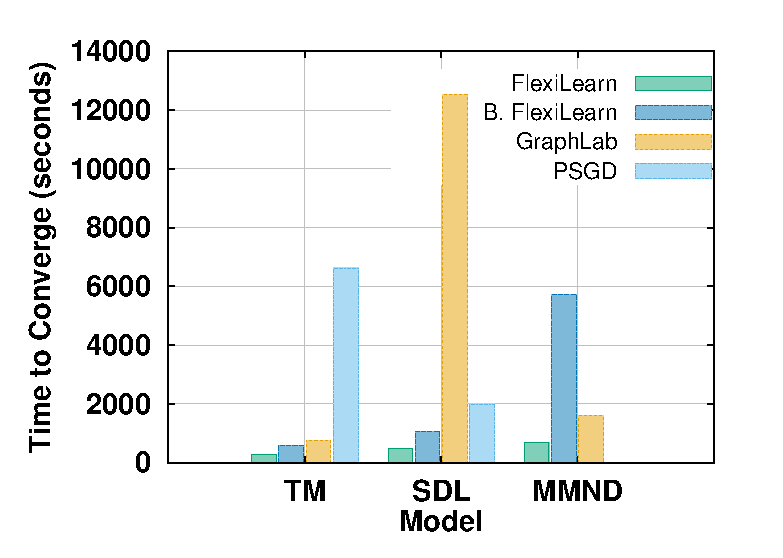
\includegraphics[width=0.46\columnwidth]{fig2/speedup.eps} &
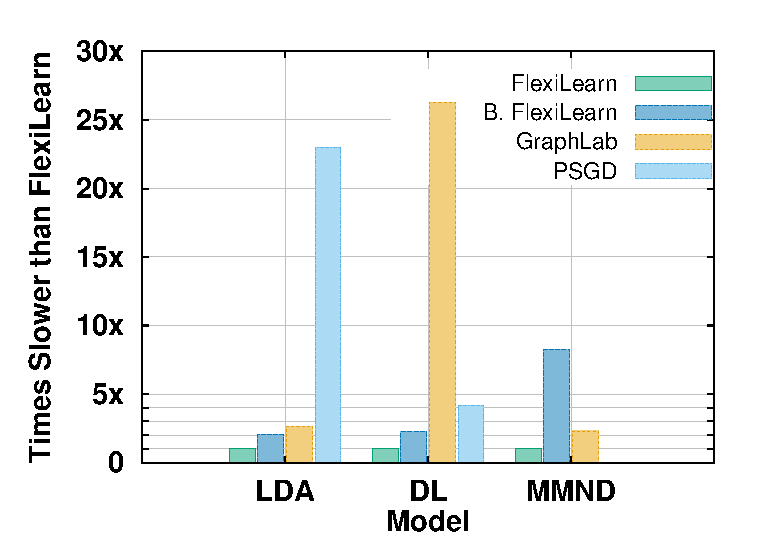
\includegraphics[width=0.46\columnwidth]{fig2/speedup2.eps} \\\hline
\end{tabular}
\vspace{-0.3cm}
\caption{\small Time taken by all methods to converge on the
three ML models, on an absolute scale (left) as well as a relative scale (right).
The methods plateau at these values in the respective plots shown
in Figure~\ref{fig:results}. The bar for \psgd is absent in the figure as it never reaches $0.059$ and stops around 
objective value $0.092$.  }
\label{fig:speed}
\end{figure}

\begin{figure}[t]
\vspace{-0.1cm}
\centering
\begin{tabular}{|c|c|}
\hline
 \multicolumn{2}{|c|} {\bf Break down of time take to finish tasks in reducer} \\
\hline
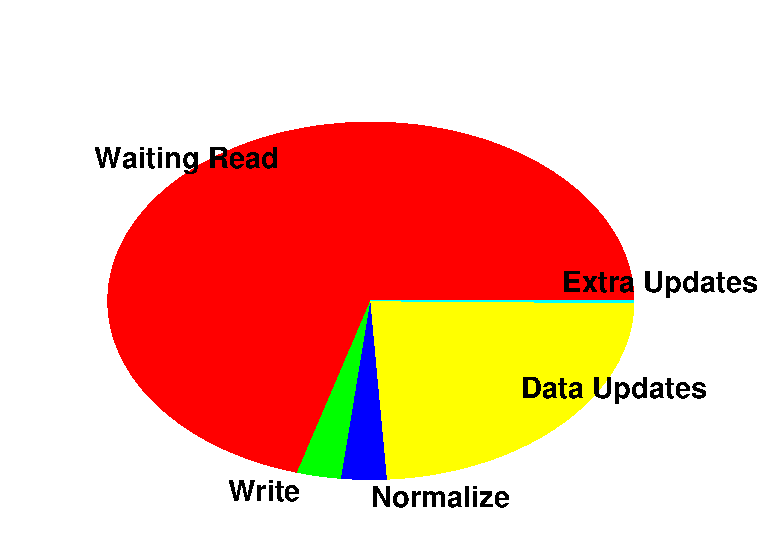
\includegraphics[width=0.46\columnwidth]{fig2/lda_piechart.eps} &
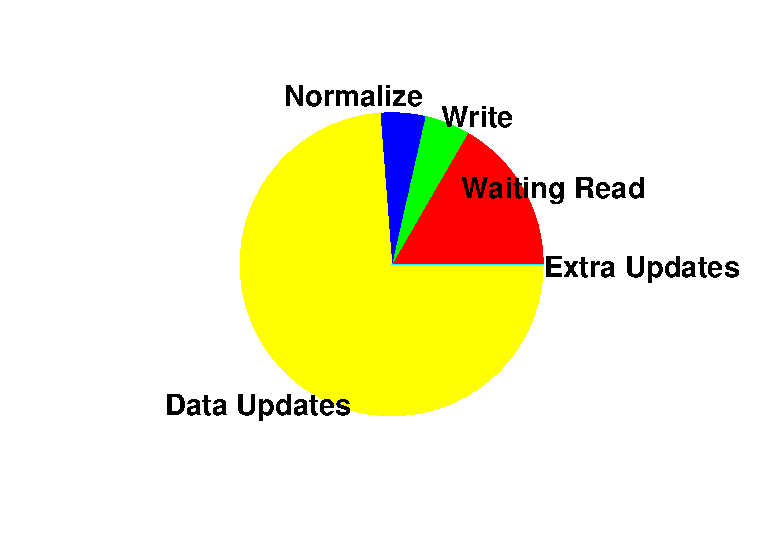
\includegraphics[width=0.46\columnwidth]{fig2/mmsb_piechart.eps} \\\hline
\end{tabular}
\vspace{-0.3cm}
\caption{\small Proportional breakup of time taken during different tasks in the 
reduce phase. The left hand graph is for \lda with 32 processors and \snytimes{32} 
dataset	and the right hand plot is for \mmsb with 32 processos and \swebgraph{8}
dataset. ``Waiting Read" is time a reducer waits to synchronize with other 
reducer to finishing 
writing its updates. ``Normalize" is the time taken to ensure the normalization constraints
for \lda and \mmsb, 
``Write" is the time taken to write the intermediate factors and output files to 
hdfs, ``Data Updates" is the time takes to perform computations on the 
data, and ``Extra Updates" is the time taken to perform extra updates while waiting 
for to synchronize with other reducers.
We can see that time for waiting to read is more than time for data updates 
in case of \lda due to distributed normalization. }
\label{fig:piechart}
\end{figure}

All four learning \schemes are evaluated on three criteria: 
1) their speed, 2) scalability (in data size as well as 
model size), and 3) quality of answers. We see that \ourmethod outperforms all 
other methods with huge margins on all three tasks and over all three criteria.


\subsection{Scalability}
Columns two, three and four in Figure~\ref{fig:results} show the scalability of different
methods in model size, number of machines and data size for all three \queries. We see
that \ourmethod performs excellently across the spectrum. 

%\vspace{-0.4cm}
%\section{Experiments}
%\vspace{-0.3cm}
%
%\begin{figure*}[t]
%\vspace{-0.4cm}
%\centering
%\begin{tabular}{|c|c|c|c|}
%\hline
%\multicolumn{2}{|c|}{\bf Topic Modeling} & {\bf Dictionary Learning} & {\bf MMND} \\
%\hline
%Convergence Plots & Scaling in \# Cores & Convergence Plots &  Convergence Plots \\
%%\multicolumn{4}{|c|}{\bf Topic Modeling} \\
%%\hline
%%Convergence Plots & \# of Topics & \# of Processors & \# of Docs \\
%\hline
%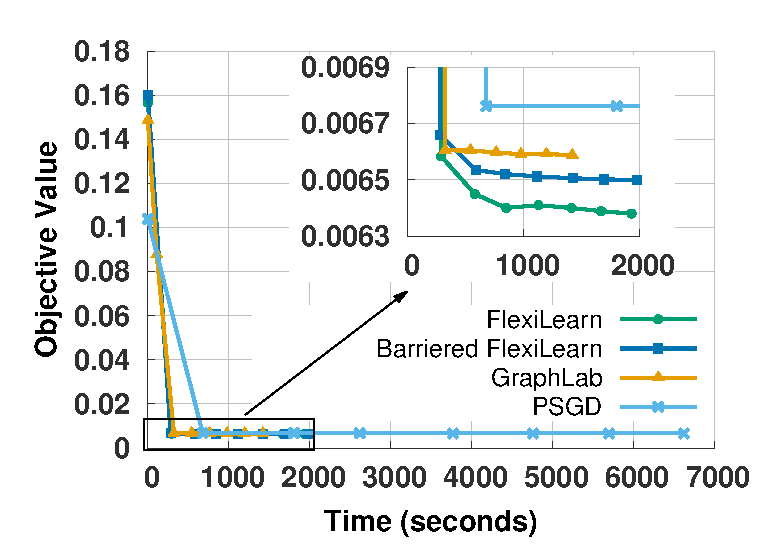
\includegraphics[width=0.23\textwidth]{fig2/lda_convergence.eps} 
%& 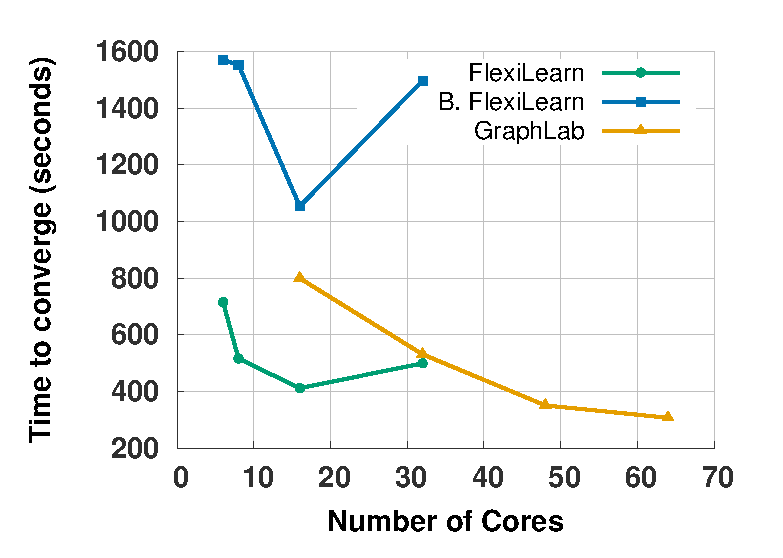
\includegraphics[width=0.23\textwidth]{fig2/lda_machines.eps} 
%& 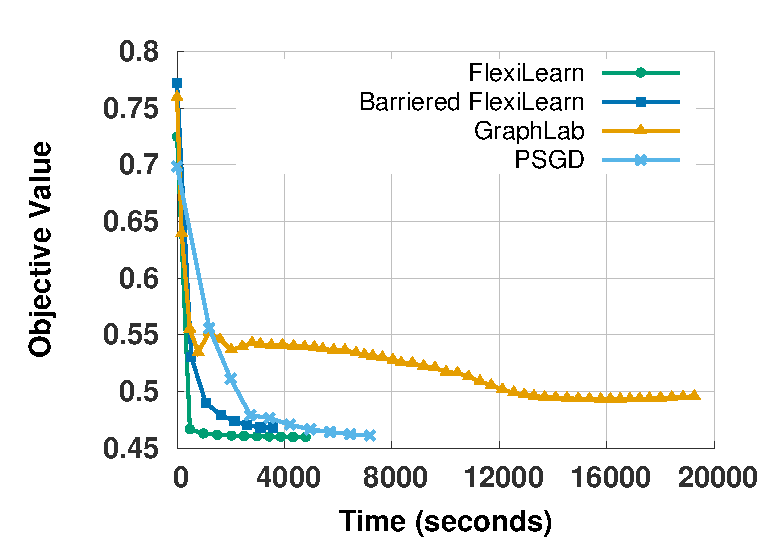
\includegraphics[width=0.23\textwidth]{fig2/dict_convergence.eps} 
%& 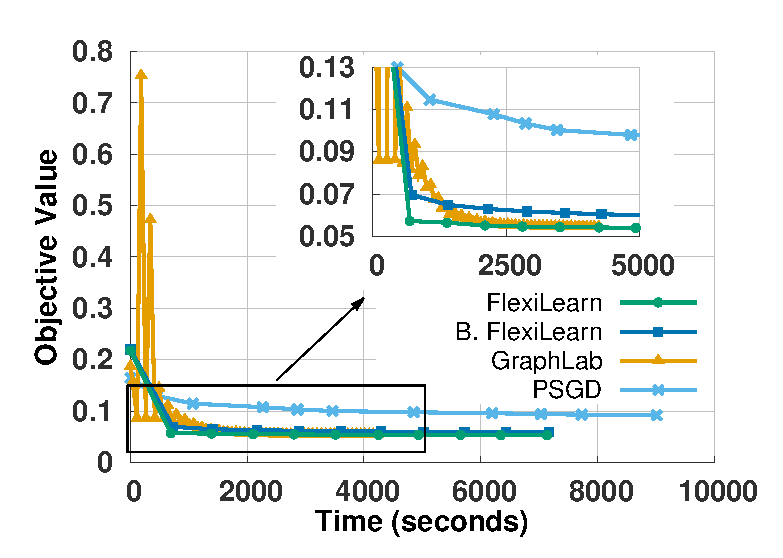
\includegraphics[width=0.23\textwidth]{fig2/mmsb_convergence.eps}  
%\\
%\hline
%%{\bf Topic Modeling} & {\bf Dictionary Learning} & \multicolumn{2}{|c|}{\bf Mixed Membership Network Decomposition} \\
%\multicolumn{4}{|c|}{\bf Topic Modeling} \\
%\hline
%Machines Needed & Scaling in \# Docs & \multicolumn{2}{|c|}{Scaling in \# Topics} \\
%\hline
%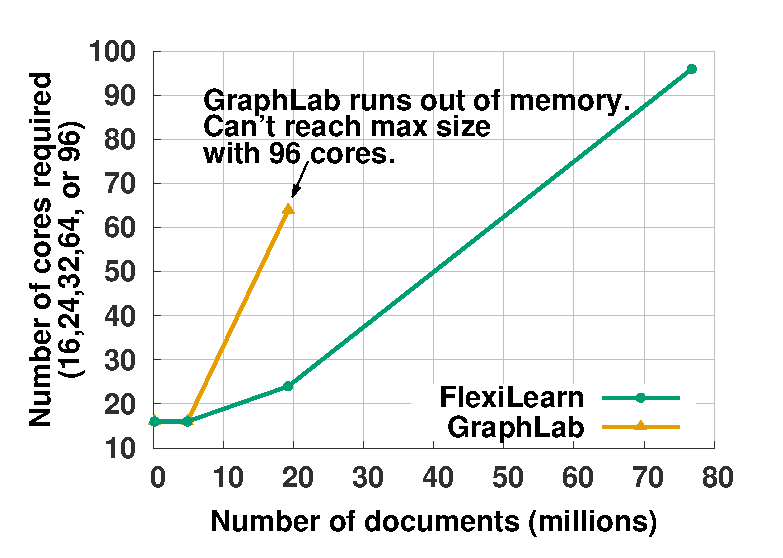
\includegraphics[width=0.23\textwidth]{fig2/lda_machines_failing.eps}
%& 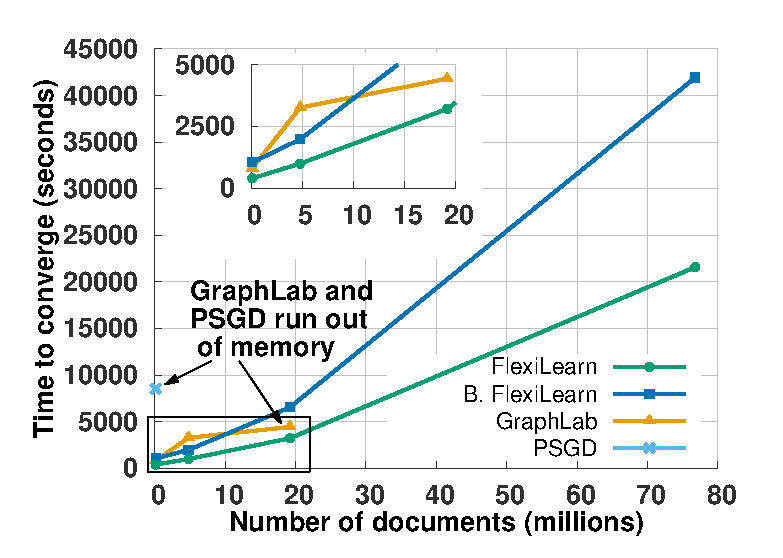
\includegraphics[width=0.23\textwidth]{fig2/lda_datasize.eps}
%& \multicolumn{2}{|c|}{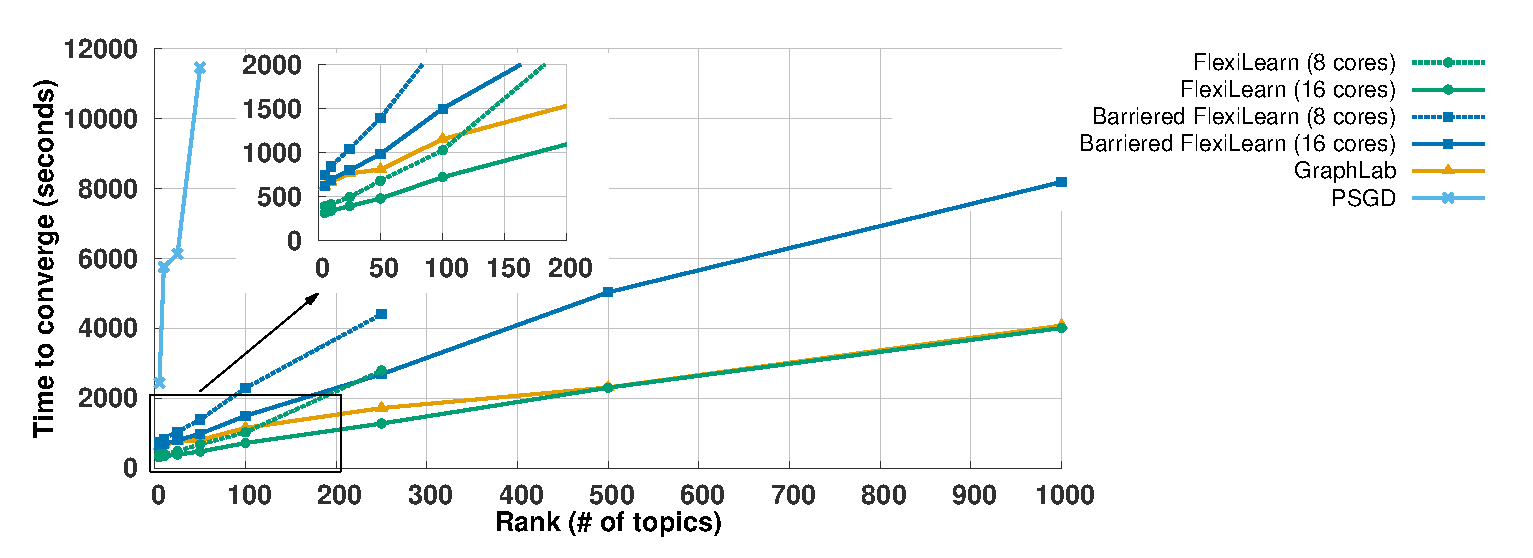
\includegraphics[width=0.46\textwidth]{fig2/lda_rankv2.eps}} \\
%\hline
%\end{tabular}
%\vspace{-0.3cm}
%\caption{\small Convergence and scalability plots for the three models (\lda, \dl, \mmsb),
%under our \ourmethod{} and baselines (\dsgd, \psgd, \graphlab). Unless otherwise stated in the plot, all methods were run with 16 cores
%and rank $K=25$. For all topic modeling plots except ``\# of Docs" and ``Machines Required", we used the NyTimes4 dataset (Table \ref{tab:dataset}).
%The convergence plots reveal the objective trajectory and final value of each method,
%while the scalability plots show how each method fares (on topic modeling) as we increase the problem rank, number of processor cores, and data size.
%In the bottom left, we also show the minimum number of machines required for a given topic modeling dataset size, for
%\ourmethod{} and \graphlab.}
%\vspace{-0.5cm}
%\label{fig:results}
%\end{figure*}

%\subsubsection{Dataset size}
\paragraph*{Dataset size}
For data size scalability experiment, we fix the number of processors at 32 
and rank at 25 for all three methods and all three applications. 
Column four of Figure~\ref{fig:results} shows the convergence time taken by the different
\schemes with respect to increasing data size. 
As explained in Section \ref{subsec:data}, we vary the data size for \lda and
\sdl by increasing the number of documents and images respectively, and for
\mmsb we increase the data size by making it denser.
%We vary the data size in two ways: 1) by 
%making the data denser e.g. increasing the number of edges in the graph (or 
%entries in the adjacency matrix ) for  
%\mmsb instead of increasing the number of vertices, 
%and 2) by increasing the dimensions of the data e.g.
%increasing the 
%number of documents. In this set of experiments we vary the \lda and \sdl data 
%size by increasing the number of documents. For \mmsb we increase the data by making it 
%denser with inclusion of more edges as explained in Section~\ref{subsec:data}. 
A subtle distinction between the two ways of increasing size is that increasing the dimension of 
the data also increases the model size e.g. for the document by word input count matrix 
for \lda, increasing the columns (number of words) increases the size of 
topic-word model parameter. 
This has bad repercussions for an approach
that is only scalable in data e.g. \psgd. 
\psgd runs out of memory very early (for data of size 6 GBs) 
in the data size experiments for \lda and \sdl since the parameters also 
increase with the increase in size of the data. For \mmsb it keeps running 
with increase in size for a while although with poor convergence. 
It doesn't reach the convergence threshold and hence is not included in the plots. 
Our \ourmethod scales well for both ways of increasing 
data size. It never runs out of memory in any of the \query types for sizes shown in the 
figure as well as is faster by at least a factor of 2. Figure~
\ref{fig:ldaMachinesNeeded} shows a comparison of number of machines needed for \ourmethod
and \graphlab for \lda. 
Figures~\ref{fig:results} and \ref{fig:ldaMachinesNeeded} combined show that not only 
\ourmethod is faster but also is more efficient with system resources.
Although like the other three \allmethods, it stores all its variables in 
memory for computation, this speed stems from the fact that \ourmethod 
is distributed over both data and model, unlike \graphlab which is distributed over 
vertices that may not correspond to a clean data and model distribution. Or unlike 
\psgd that only is distributed over data and not model.  
While any of these systems could be modified to spill onto disk for large
models, this would only computation significantly.
%\alex{we need to be more concrete here and explain that we are all memory based
%systems}


%\paragraph{Model parameters}
\paragraph*{Model parameters}
As we want to include more topics in our topic model or more basis vectors in
our \sdl model, the number of variables we have to learn increases
significantly.
%The model parameter are the types of variables that arise as a construct of the
%model (Section~\ref{sec:problem}). For example, the number of topics 
%in \lda or the number of basis vectors in \sdl is a construct of the model.  
Column two of Figure \ref{fig:results} shows how different methods scale in
rank for all three applications. For this set of experiments we fix number of
processors as 16 for all 
\allmethods and \queries. 
The datasets used are \snytimes{4}, \swebgraph{1}, and \imagenet for \lda,
\mmsb and \sdl respectively.
Here again we see that \ourmethod is faster to converge than all the other
\allmethods. The difference in convergence rate of \graphlab and \ourmethod is especially stark
for \sdl. The reason for this is that \graphlab oscillates by huge margins for this problem as
seen in Figure~\ref{fig:results}, second row, first column. 
\psgd runs out of memory quite early (for rank 100) as expected for \lda and \sdl.
Since the dimensions of the \mmsb data are smaller (281,904) that \lda (1,200,000) or \sdl
(1,261,406), \psgd runs out of memory a little later (for rank 200) for this \mmsb \query. 

%\paragraph{Processors}
\paragraph*{Processors}
Column three of Figure \ref{fig:results} shows the effects of varying number of processors for a fixed data and model size.
We have set rank as 25 and used \snytimes{32}, \swebgraph{8}, and \simagenet{4}
as data sets for \lda, \mmsb, and \sdl. 
In the case of \sdl and \mmsb, \ourmethod performs significantly better compared to others.
For these set of experiments \psgd doesn't converge to the optimal point as more 
machines are added due to its bad averaging guarantees
on non-convex problems and is significantly slower too.
%since all the variable after independently being computed in the 
%update phase on $d$ reducers ($d=32$ here) are passed through a single 
%reducers for averaging and thus
%creating a bottleneck.  
We scale well in terms of processors needed for larger data sets for \lda compared to \graphlab.
We observe that for small data sizes \ourmethod eventually starts giving 
worse returns with increasing processors in case of \lda and its curve
is worse than \graphlab. But for larger datasets \ourmethod
has the best curve. This is because on smaller datasets time
taken to synchronize among the reducers dominates the time taken to perform
computations on the data. 

This fact is also illustrated in Figure~\ref{fig:piechart}. 
Figure~\ref{fig:piechart} shows a break down of the percentage of time each reducer
spends on different tasks. For \lda every reducer has to perform 
distributed projections, and to achieve this a reducer has to poll 
all the other reducers at the end of every subepoch, leading to 
extra waiting compared to a non-distributed projection.  
The effects of this wait is more pronounced for \dsgd as it performs much worse 
(Figure~\ref{fig:results}, column three, row one). Our method due to its provably correct Always-On property
mitigates the ill effects of sync-waits by doing more work.
For \mmsb most 
time is spent on computation because less 
synchronization is necessary. 
%Though there is still synchronization happening between two 
%consecutive blocks in a sub-epoch where reducer in block $i$ is waiting for reducer in 
%block $i+1$ to finish so that reducer in $i$ can move to block $i+1$ 
%in the next sub-epoch.
The actual number of data points updated in the ``Extra Updates" are 950,760 (of $10.3*10^9$ 
total data points) and 14,556,089 (of $3.2*10^9$ total data points) per 
reducer (in all 32 reducers) per epoch. 

\subsection{Overall convergence speed}
Figure~\ref{fig:speed} shows convergence times 
for \ourmethod{}, \dsgd, \psgd, and \graphlab over the three 
models: \lda, \mmsb and \dl. \ourmethod{} is faster
by anywhere between $2.6\times$ (vs \graphlab on \lda) 
to $26.2\times$ (vs \graphlab on \sdl). This clearly is due to the Always-On 
property of \ourmethod.
The number of reducers used is 16 and the datasets are \snytimes{4}, \swebgraph{1} and 
\imagenet. 
%\begin{figure}[t]
%\vspace{-0.4cm}
%\centering
%\begin{tabular}{|c|c|}
%\hline
% \multicolumn{2}{|c|} {\bf Time taken to converge} \\
%\hline
%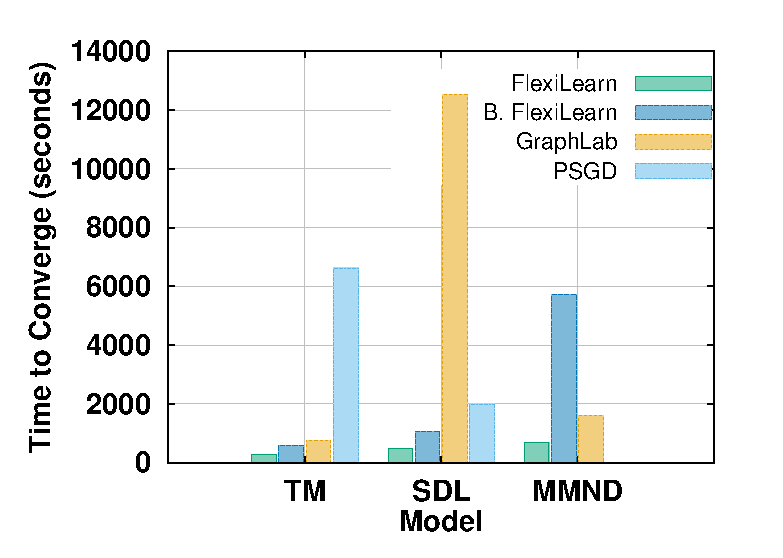
\includegraphics[width=0.46\columnwidth]{fig2/speedup.eps} &
%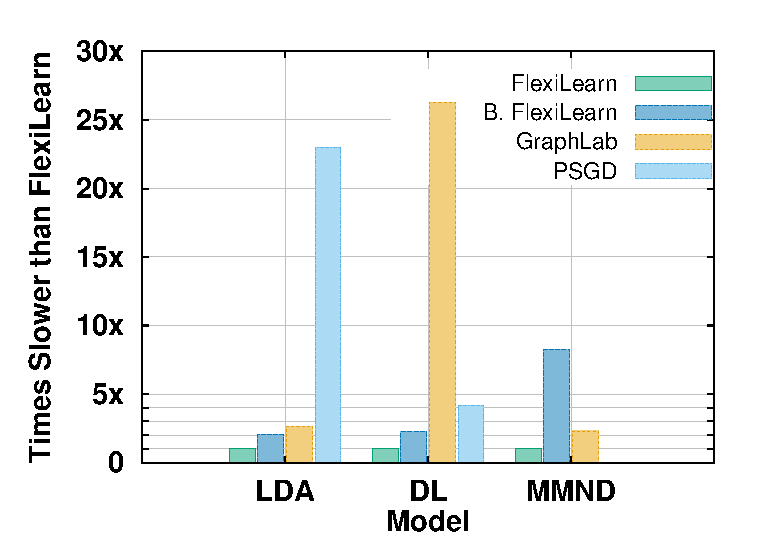
\includegraphics[width=0.46\columnwidth]{fig2/speedup2.eps} \\\hline
%\end{tabular}
%\vspace{-0.3cm}
%\caption{\small Time taken by all methods to converge on the
%three ML models, on an absolute scale (left) as well as a relative scale (right).
%The methods plateau at these values in the respective plots shown
%in figure~\ref{fig:results}. The bar for \psgd is absent in the figure as it never reaches $0.059$ and stops around 
%objective value $0.092$.  }
%\label{fig:speed}
%\end{figure}

\subsection{Convergence quality}
Last we test the convergence rates of the methods.
Here we use  16 processors, set rank to 25, and  use the
\snytimes{4}, \swebgraph{1}, and \imagenet for \lda, \mmsb and \sdl respectively.
%Though \graphlab is large scale and is a distributed work load system, it has no theoretical guarantees. 
This shows up in the quality of answers we get. \ourmethod is distributed, faster,
better scalable, and gives higher quality of answers. Figure~\ref{fig:results}, 
column one shows the convergence curve for all the approaches on all three problems.
\ourmethod converges to a better value more quickly than all of the other methods.
The higher quality of results stems from the fact that \ourmethod is 
guaranteed to be correct theoretically. \graphlab oscillates quite a lot for \mmsb and \sdl. 
This is due to  the fact that it updates vertices in partitioned sets without any guarantees
for the constraints (as discussed in Section~\ref{sec:complexQues}).
%\graphlab oscillation reasons and patterns, \dsgd and \psgd converges to a poor
%quality,
\subsection{Why \ourmethod succeeds}
The reason \ourmethod performs better than state of the art competitors on all
three criteria and on all three problems can be attributed to the following :
\begin{itemize}[noitemsep,topsep=1.5pt,parsep=1.5pt,partopsep=1.5pt] 
\item Unlike \psgd, it is distributed over data as well as model. This gives \ourmethod 
atleast twice the speed as well as scalability compared to \psgd 
\item Unlike \graphlab, it is theoretically grounded. This gives \ourmethod a guarantee 
for high quality answers
\item Unlike \dsgd it does not waste time while waiting to synchronize. This makes it 
more scalable (as we saw in case of machine scalability) and faster by several factors of
magnitude.
\end{itemize}
%Put a plot of waiting times in different concstraints case and argue why it
%helps here.
